\chapter{LSPE/Strip}

In this chapter LSPE, a next generation CMB experiment, is briefly
introduced. In particular, we focus our attention on Strip, the standalone
ground-based telescope of the LSPE project. This instrument constitutes the
case study to which our novel approach for atmospheric effects forecasting
in CMB experiments is applied.

First, LSPE as a whole is described. Then, some Strip technical details and
the observation site to which the instrument will be deployed are covered.

\section{The LSPE Experiment}

The \emph{Large Scale Polarization Explorer} (LSPE) (8446 SPIE 2012)
project aims either to detect the polarization B-modes of the cosmic
microwave background or to constrain the scalar-to-tensor ratio (see
\autoref{ss:inflation_perturbations}) to $r \simeq 0.03$ at the
\SI{99.7}{\percent} confidence level. The polarized emission of our galaxy
at large angular scales from the Earth's Norther Hemisphere will also be
studied in a range of frequencies between \SIlist{40;250}{\giga\hertz}.

LSPE is composed of two experiments:

\begin{itemize}
        \item \textbf{SWIPE:} a balloon borne instrument consisting of
        three arrays of \num{110} large throughput multi-mode bolometers
        centered at the frequencies \SIlist{140;220;240}{\giga\hertz}. It
        will be launched from the Svalbard Islands and will survey the Norther
        Sky in a long duration flight during the Artic Winter;

        \item \textbf{Strip:} a ground-based telescope that will be
        deployed to the \emph{Observatorio del Teide} in Tenerife and will
        provide approximately the same sky coverage of SWIPE, with an
        observed sky overlap \SI{> 80}{\percent}.
\end{itemize}

The LSPE experiment will be operative by the end of the year 2022.

\section{The Strip Instrument}

\begin{figure}
        \centering
        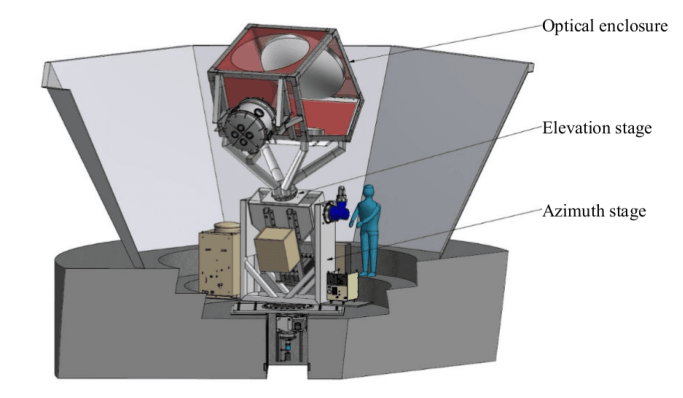
\includegraphics[width=\textwidth]{LSPE-Strip-optical-system}
        \caption{LSPE/Strip Optical System}
        \label{fig:lspe-strip_optical_system}
\end{figure}

\begin{figure}
        \centering
        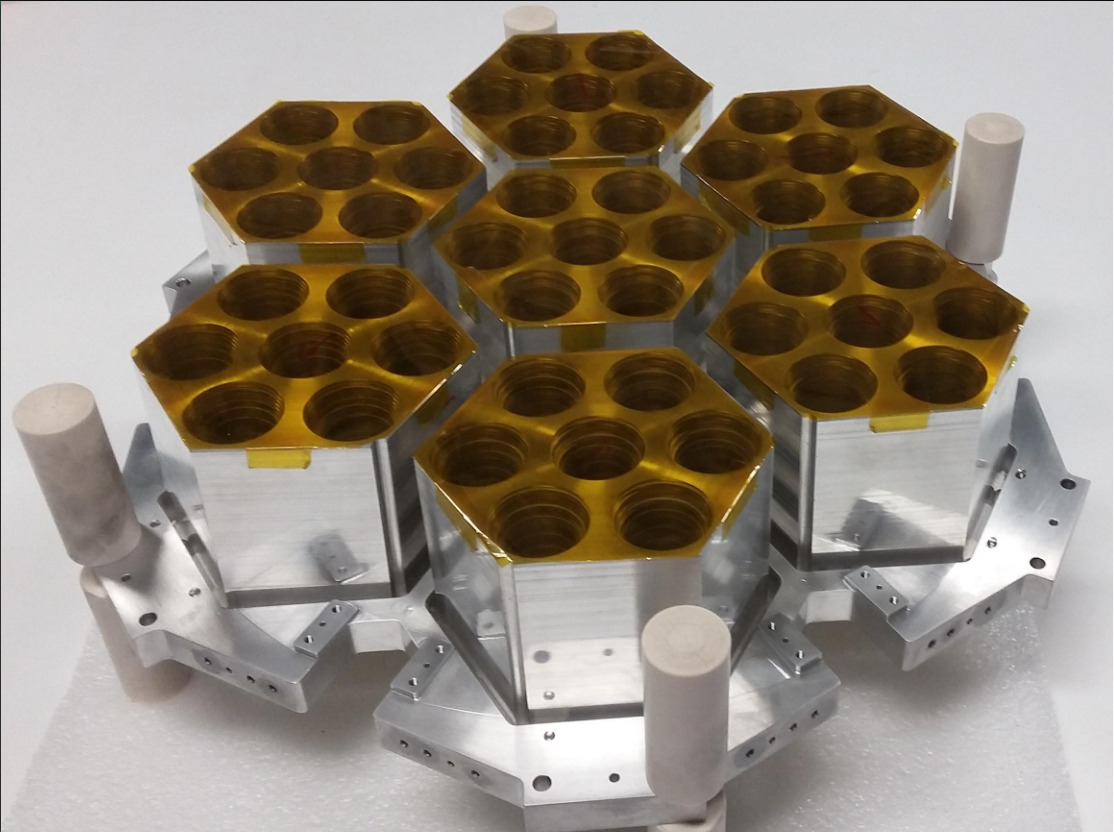
\includegraphics[width=\textwidth]{strip-focal-plane}
        \caption{Strip focal plane}
        \label{fig:strip_focal_plane}
\end{figure}

\subsection{The Observation Site}

The Strip instrument will be deployed to the \emph{Observatorio del Teide}
in the city of Iza\~na, in Tenerife Island, Spain (\ang{28;18;04} N,
\ang{16;30;38} W) (see \autoref{fig:observatorio_teide}). The astronomical
observatory is located on Mount Teide at \SI{2390}{\meter} above sea level
and it has been operated by the \emph{Instituto de Astrof\'isica de
Canarias} since 1964.

The Observatory's geographical location, combined with the excellent
quality of the sky for astronomy, led to Teide Observatory being dedicated
mainly to  the study of the sun. However, Teide Observatory hosted and
still hosts different CMB experiments.
The \emph{Tenerife Experiment} (1984) by Jodrell Bank (of the University of
manchester) was the first CMB experiment to be installed at the
observatory. It measured CMB temperature anisotropies on angular size of
\ang{5}. Currently the observatory hosts the \emph{Multi Frequency
Instrument} (MFI), the \emph{Thirty Gigahertz Instrument} (TGI) and the
\emph{Forty Gigahertz Instrument} (FGI) of the \emph{Q-U-I JOint TEnerife
CMB} (QUIJOTE-CMB) experiment by the Instituto de Astrof\'isica de
Canarias. QUIJOTE experiment aims to characterize the
polarization of the CMB radiation in the frequency range
\SIrange{10}{42}{\giga\hertz}. The Strip instrument will join the
international efforts to detect the B-modes of the CMB polarization,
observing the microwave sky from the same site.

The characteristic geographical and climatic non-homogeneity typical of
relatively small islands constitutes a challenge for the estimate of the
systematics linked to atmospheric effects. This problem will be tackled in
the next chapters of this thesis.



\begin{figure}
        \centering
        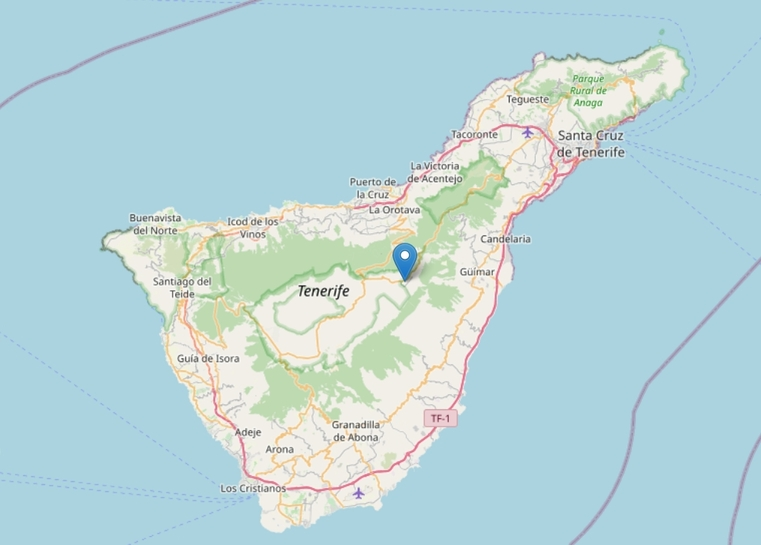
\includegraphics[width=\textwidth]{observatorio_teide}
        \caption{Observatorio del Teide}
        \label{fig:observatorio_teide}
\end{figure}

